\begin{frame}{A pathological problem example}


An input sequence:

\vspace{1em}

\begin{tabular}{|c|c|c|c|c|c|c|c|c|c}
	\hline  marker & 0&  1&  0&  $\hdots$& 0 & 1 & 0 & 0  \\ 
	  value & 0.3&  \textbf{0.7}&  0.1&  $\hdots$& 0.2& \textbf{0.4} & 0.6& 0.9  \\ 
	\hline 
\end{tabular}

\vspace{1em}
The predicted output should be the sum of the two one marked positions (1.1). 
\pause
\vspace{1em}
\begin{block}{Why is this a difficult problem?}
	\pause
	Because of it's long time dependencies.
\end{block}

\end{frame}

\begin{frame}{Gradient}
	Consider a $\net{RNN}=\langle\set{W},\set{B},\sigma(\cdot),F(\cdot)\rangle$. Let $L_t:\mathbb{R}^o \times \mathbb{R}^o \rightarrow \mathbb{R}$ a loss function and  $g_t(\cdot):\mathbb{R}^{\mathcal{N}(\set{W})+\mathcal{N}(\set{B})} \rightarrow \mathbb{R}$ be the function defined by
	$$g_t(\set{W},\set{B}) \triangleq L_t(F(\vec{y}^t(\set{W},\set{B})))$$
	and $$g(\set{W},\set{B}) \triangleq \sum_{t=1}^T g_t(\set{W},\set{B})$$
	
	
	\begin{align}
	\frac{\partial g}{\partial \mat{W}^{rec}} &= \sum_{t=1}^T \nabla L_t^T \cdot J(F) \cdot \frac{\partial \vec{y}^t}{\partial \vec{a}^t} \cdot \frac{\partial \vec{a}^t}{\partial \mat{W}^{rec}}\\
	&= \sum_{t=1}^T\frac{\partial g_t}{\partial \vec{a}^t} \cdot \frac{\partial \vec{a}^t}{\partial \mat{W^{rec}}}
	\end{align}
\end{frame}
\begin{frame}

	Let's see how to compute $\frac{\partial \vec{a}^t}{\partial \mat{W}^{rec}}$.
	
	Let's consider a single output unit $u$, and a weight $w_{lj}$, we have
	
	\begin{align}
	\label{sum_over_time}
	\frac{\partial a^t_u}{\partial w_{lj}} &= \sum_{k=1}^t \frac{\partial a_u^t}{\partial a^k_l} \cdot \frac{\partial a^k_l}{\partial w_{lj}}\\
	&= \sum_{k=1}^t \delta^{tk}_{lu} \cdot \phi_j^{t-1}
	\end{align}
	where
	\begin{equation}
	\delta_{lu}^{tk} \triangleq \frac{\partial a_u^t}{\partial a^k_l}.
	\end{equation}
	
	Let $P(l)$ be the set of parents of neuron $l$, defined as the set of parents in the unfolded network.
	
	\begin{equation}
	\delta_{lu}^{tk} = \sum_{h\in P(l)} \delta_{hu}^{tk} \cdot \sigma'(a_h^{t-1})\cdot w_{hl}
	\end{equation}
\end{frame}
\begin{frame}
	
	\tikzstyle{rnn_style}=[->,shorten >=1pt,auto,node distance=1.5cm,
	thick,
	neuron/.style={circle,fill=white!50,draw,minimum size=0.7cm,font=\sffamily\normalsize},
	missing/.style={circle,fill=white!50,draw=none,minimum size=0.7cm,font=\sffamily\Huge\bfseries},
	label/.style={node distance=1.2cm,rectangle,fill=white!50,draw=none,minimum size=0.7cm,font=\sffamily\normalsize},
	thick_edge/.style={line width=1.2pt},
	thin_edge/.style={line width=0.5pt}
	]
	\begin{figure}
		\centering
		\resizebox{5cm}{!}{
		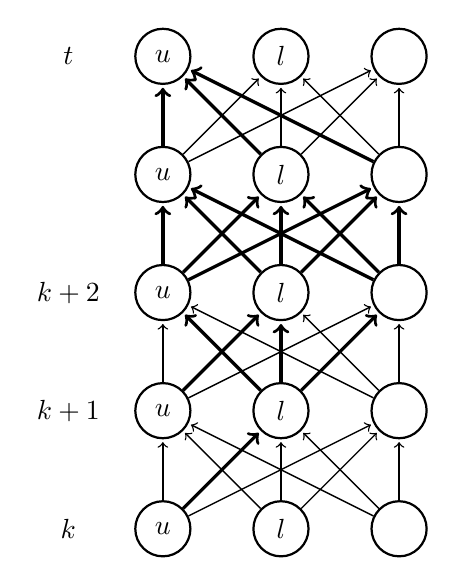
\begin{tikzpicture}[rnn_style]
		
		
		\node[neuron]    (x1)[]   {$u$};
		\node[neuron]    (x2)[right of=x1]   {$l$};
		\node[neuron]    (x3)[right of=x2]   {};
		\node[label]     (xl)[left of=x1] {$t$};
		
		\node[neuron]    (h1)[below of =x1]   {$u$};
		\node[neuron]    (h2)[right of=h1]   {$l$};
		\node[neuron]    (h3)[right of=h2]   {};
		\node[label]     (hl)[left of=h1] {$\hdots$};
		
		\node[neuron]    (y1)[below of=h1]   {$u$};
		\node[neuron]    (y2)[right of=y1]   {$l$};
		\node[neuron]    (y3)[right of=y2]   {};
		\node[label]     (yl)[left of=y1] {$k+2$};
		
		
		\node[neuron]    (z1)[below of=y1]   {$u$};
		\node[neuron]    (z2)[right of=z1]   {$l$};
		\node[neuron]    (z3)[right of=z2]   {};
		\node[label]     (zl)[left of=z1] {$k+1$};
		
		\node[neuron]    (w1)[below of=z1]   {$u$};
		\node[neuron]    (w2)[right of=w1]   {$l$};
		\node[neuron]    (w3)[right of=w2]   {};
		\node[label]     (wl)[left of=w1] {$k$};
		
		
		%   \node[label]      (lu)[left of=u] {$u$};
		%   \node[label]      (ll)[left of=z1] {$l$};
		
		
		\path[->] (h1) edge [thick_edge]  (x1)
		(h1) edge [thin_edge]   (x2)
		(h1) edge [thin_edge]   (x3)
		(h2) edge [thick_edge]  (x1)
		(h2) edge [thin_edge]   (x2)
		(h2) edge [thin_edge]   (x3)
		(h3) edge [thick_edge]  (x1)
		(h3) edge [thin_edge]   (x2)
		(h3) edge [thin_edge]   (x3);
		
		\path[->] (y1) edge [thick_edge]   (h1)
		(y1) edge [thick_edge]   (h2)
		(y1) edge [thick_edge]   (h3)
		(y2) edge [thick_edge]   (h1)
		(y2) edge [thick_edge]   (h2)
		(y2) edge [thick_edge]   (h3)
		(y3) edge [thick_edge]   (h1)
		(y3) edge [thick_edge]   (h2)
		(y3) edge [thick_edge]   (h3);
		
		
		\path[->] (z1) edge [thin_edge]   (y1)
		(z1) edge [thick_edge]  (y2)
		(z1) edge [thin_edge]   (y3)
		(z2) edge [thick_edge]  (y1)
		(z2) edge [thick_edge]  (y2)
		(z2) edge [thick_edge]  (y3)
		(z3) edge [thin_edge]   (y1)
		(z3) edge [thin_edge]   (y2)
		(z3) edge [thin_edge]   (y3);
		
		\path[->] (w1) edge [thin_edge]   (z1)
		(w1) edge [thick_edge]  (z2)
		(w1) edge [thin_edge]   (z3)
		(w2) edge [thin_edge]   (z1)
		(w2) edge [thin_edge]   (z2)
		(w2) edge [thin_edge]   (z3)
		(w3) edge [thin_edge]   (z1)
		(w3) edge [thin_edge]   (z2)
		(w3) edge [thin_edge]   (z3);
		
		
		\end{tikzpicture}
		}
		\caption{Nodes involved in $\frac{\partial a^t_u }{\partial a^k_l}$.}
		\label{deriv_arcs_rnn}
	\end{figure}
\end{frame}
\begin{frame}
	In matrix notation we have:
	
	\begin{equation}
	\frac{\partial \vec{a}^t}{\partial \mat{W}^{rec}} = \sum_{k=1}^t \frac{\partial \vec{a}^t}{\partial \vec{a}^k} \cdot \frac{\partial^+ \vec{a}^k}{\partial \mat{W}^{rec}}
	\end{equation}
	
	
	\begin{equation}
	\frac{\partial^+ a^{k}}{\partial \mat{W}_j^{rec}} =
	\begin{bmatrix}
	\phi_j^{k}    & 0                & \cdots      & \cdots       & 0  \\
	0               & \phi_j^{k}     & \cdots      & \cdots       & 0  \\
	\vdots          & \vdots           & \ddots      & \vdots       &\vdots\\
	0               & \cdots           & \cdots      & \cdots       & \phi^{k}_{j}
	\end{bmatrix}
	\end{equation}
	
	\begin{equation}
	\triangleq \mat{\Delta}^{tk}
	\end{equation}
	
	\begin{align}
	\mat{\Delta}^{tk} &= \mat{\Delta}^{t(k+1)} \cdot diag(\sigma'(\vec{a}^k)) \cdot \mat{W}^{rec} \\
	&= \prod_{i=t-1}^{k} diag(\sigma'(\vec{a}^i)) \cdot \mat{W}^{rec}
	\label{rnn_delta}.
	\end{align}
	
	The derivatives with respect to the other variables are computed in a similar fashion

	
\end{frame}


\begin{frame}{Vanishing gradient: an upper bound}
	\begin{equation}
	\frac{\partial \vec{a}^t}{\partial \vec{a}^k} = \prod_{i=t-1}^{k}  diag(\sigma'(\vec{a}^i)) \cdot \mat{W}^{rec}.
	\label{eq:temporalComponent}
	\end{equation}
	
	Taking the singular value decomposition of $\mat{W}^{rec}$:
	\begin{equation}
	\mat{W}^{rec} =  \mat{S}\cdot\mat{D}\cdot\mat{V}^T
	\end{equation}
	where $\mat{S},\mat{V}^T$ are squared orthogonal matrices and $\mat{D}\defeq diag(\mu_1, \mu_2,...,\mu_r)$ is the diagonal matrix containing the singular values of $\mat{W}^{rec}$.
	Hence:
	\begin{equation}
	\frac{\partial \vec{a}^t}{\partial \vec{a}^k} = \prod_{i=t-1}^{k}  diag(\sigma'(\vec{a}^i)) \cdot \mat{S}\cdot \mat{D} \cdot \mat{V}^T
	\end{equation}
\end{frame}
\begin{frame}
	Since $\mat{U}$ and $\mat{V}$ are orthogonal matrix, hence $$\norm{\mat{U}}_2=\norm{\mat{V}^T}_2 = 1,$$ and $$\norm{diag(\lambda_1, \lambda_2,...,\lambda_r)}_2 \leq \lambda_{max},$$ we get
	\begin{align}
	\norm{\frac{\partial \vec{a}^t}{\partial \vec{a}^k}}_2 &= \norm{ (\prod_{i=t-1}^{k} diag(\sigma'(\vec{a}^i)) \cdot \mat{S}\cdot \mat{D} \cdot \mat{V}^T)}_2\\
	&\leq (\sigma'_{max} \cdot \mu_{max})^{t-k-1}
	\end{align}
\end{frame}

